\section{研究背景和动机}
\label{chap:zigzag:motivation}

本章主要介绍研究背景及研究动机,主要包括基于主动丢包的时间隐通道可行性分析,对Zigzag矩阵应用在码字-符号转换中的意义,及CRC校验如何提高时间隐通道的鲁棒性几个方面。结合\nref{chap:backinfo}对时间隐通道,及VoLTE视频通话场景的信道分析,参照\nref{chap:analyze}部分时间隐通道检测方法的测试,充分利用时间隐通道的构建基础,设计具有实际应用价值的构建方法,是本章的主要工作。

\subsection{基于主动丢包构建时间隐通道}
\label{chap:zigzag:motivation:dropout}
如图\nref{fig:2:pmf-dropout},VoLTE网络噪声中,长度为1的离散丢包占据总量的50\%左右。并且经过\nref{chap:analyze:result}实验的检验,当时间隐通道的主动丢包率降低到一定程度,即可规避现有的检测方法。因此,基于主动丢包的时间隐通道,在基本构造原理上依然可行。

对于隐通道的通信双方来说,如何有效识别数据包是一个非常重要的问题。在VoLTE中,可以有效利用RTP头中的Sequence Number字段,识别一次通话中数据包的唯一性。如图\nref{fig:2:rtp-header},数据包序号字段占据16 bit,最大可达到65536。正如\nref{chap:backinfo:rtp:dropout}对RTP丢包处理的描述,Sequence Number字段的作用,是识别一次通话中的数据包顺序,按照正确的顺序将负载提供给应用层。

基于数据包序号构建基于主动丢包的时间隐通道,具有以下优势:
\begin{itemize}
    \item 数据包序号具有传输同步能力,隐通道的传输过程以序号为参照时钟,无需时钟参照,简化了传输流程;
    \item 主动丢包行为不依赖数据包顺序,网络噪声中的乱序无法影响隐通道鲁棒性,防守方的数据包重排序也无法破坏隐通道;
    \item 防守方在防御时需要考虑对用户体验的影响,因此构造数据包填充丢包位置,对用户来说是可察觉的异常现象,一定程度上保证了丢包位置的传递;
    \item 如果防守反对数据包序号字段进行了覆写,则时间戳增长的线性关系被破坏,接收方可以监测到异常,并终止会话。
\end{itemize}

\subsection{ZigZag矩阵及其特征}
\label{chap:zigzag:motivation:zigzag}

\insertFigure{
	\begin{figure}
		\centering
        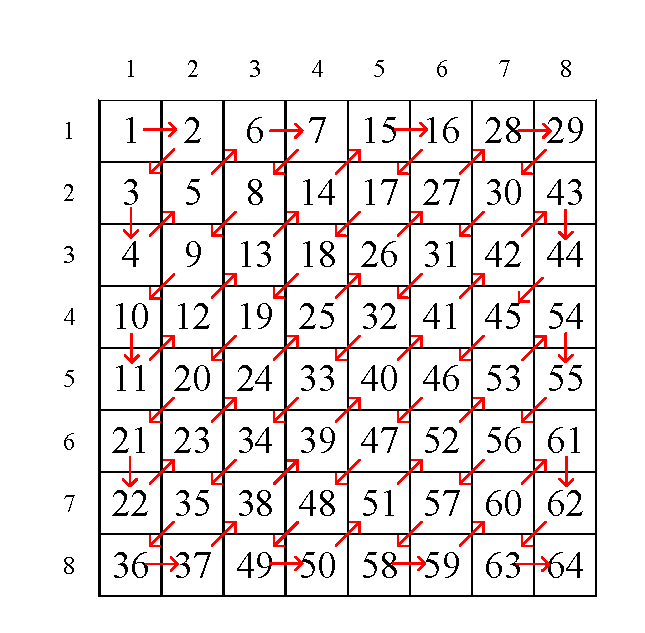
\includegraphics[width=0.6\textwidth]{chapters/chapter4/figures/zigzag-matrix.pdf}
        \caption{$8\times 8$的Zigzag矩阵示意图}
        \label{fig:4:zigzag-matrix}
	\end{figure}
}

Zigzag矩阵的排布方式,区别于常见的行优先或列优先,采用的是对角线折返的方式,不具备明显的线性关系。\nupcite{ji2015a,zaidee2006content,yang2018adaptive,li2019a}如图\nref{fig:4:zigzag-matrix}所示,矩阵中元素的坐标$(x,y)$,与元素的对应关系,由矩阵的规模决定。对于$L_{Codeword}=8$的时间隐通道来说,码字可以按照4 bit切分为上半部及下半部。参照Zigzag映射矩阵的定义,$(Codeword_{4~7},Codeword_{0~3})$可以对应到序号$Symbol$。

另一方面,Zigzag矩阵作为映射矩阵,其起始值支持用户设定,隐通道的双方可以约定一个安全的起始值,提高隐通道的保密性。即使防守方破解了隐通道的工作模式,并按照相同的解调方式,破解隐蔽消息,则需要对所有的可行解进行推测,提高了计算复杂度。随着矩阵规模的增大,矩阵中元素的排布关系会更加复杂,满足了隐通道的保密性要求。

\subsection{CRC数据校验策略}
\label{chap:zigzag:motivation:crc}

CRC是Cyclic Redundancy Check的缩写,全称为循环冗余校验码,在计算机网络及数据存储中有广泛应用。CRC作为散列函数的一种,可以生成数据的唯一摘要,根据位数的区别,常用的模式为CRC16及CRC32,更多的位数可以保证更低的冲突概率。在本时间隐通道中,CRC主要用于校验码字的正确性,无法使用全部的CRC校验值,因此,CRC16产生的结果可以基本满足校验的需求。

\insertFigure{
	\begin{figure}
		\centering
        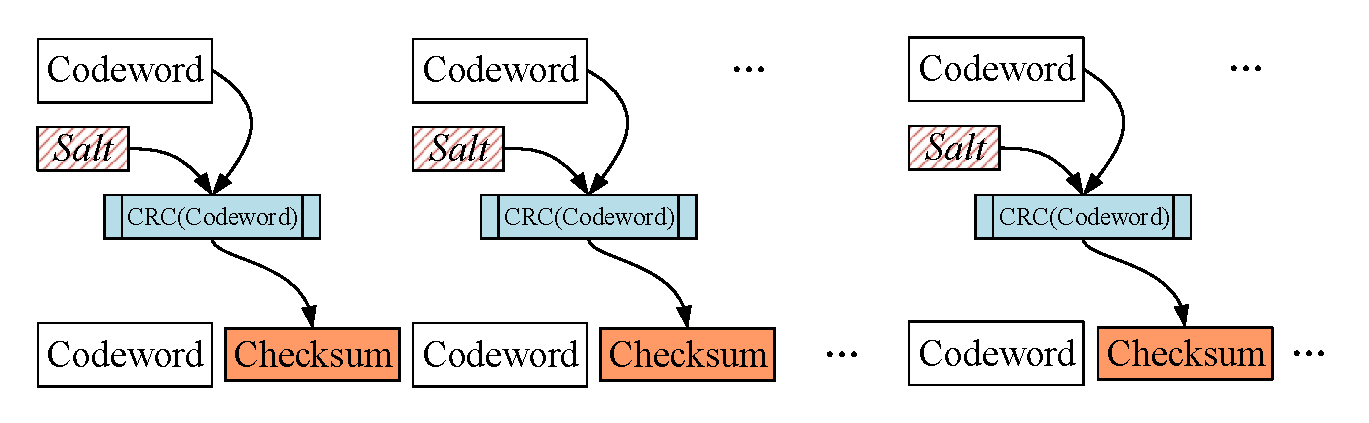
\includegraphics[width=0.98\textwidth]{chapters/chapter4/figures/insert-crc.pdf}
        \caption{CRC校验添加模式示意图}
        \label{fig:4:insert-crc}
	\end{figure}
}

如图\nref{fig:4:insert-crc},在每个数据码字之后,追加一个校验码字,通过校验码字区分噪声及信号。在CRC的参数方面,除了当前待验证的码字,额外引入$Salt$变量,增加计算结果的随机性及保密性。$salt$由两部分组成,一部分是用户自定义的私有值,一部分是RTP数据包头中导出的随机字段。在掺杂网络噪声的场景中,借助散列函数的单向性,提高防守方破解隐蔽消息的难度及计算量。

\insertTable{
	\begin{table}[]
      \centering
      \caption{添加CRC校验后的码字密度表}
      \label{tab:4:codeword-density}
          \begin{tabular*}{0.98\textwidth}{@{\extracolsep{\fill}}ccccc}
            \toprule
            $L_{Codeword}$ (bit) & 码字及校验长度 (bit) & 数据包数 & 校验编码利用率 & 总体编码利用率 \\
            \midrule
            6 & 12 & 128 & 65.6\% & 83.6\% \\
            7 & 14 & 256 & 66.4\% & 82.4\% \\
            8 & 16 & 512 & 68.0\% & 81.1\% \\
            9 & 18 & 1024 & 64.5\% & 82.2\% \\
            10 & 20 & 2048 & 62.8\% & 81.3\% \\
            11 & 22 & 4096 & 62.9\% & 81.9\% \\
            12 & 24 & 8192 & 63.2\% & 81.8\% \\
            \bottomrule
          \end{tabular*}
    \end{table}
}

通过组合码字及CRC校验信息,等价于形成了一个超长码字,并且码字中自带校验信息。采取数据及校验分别传输的方式,能够有效提高码字的传输效率,同时保证信道资源的利用率。如表\nref{tab:4:codeword-density},按照一个数据码字对应一个校验码字的方式,传输一个码字,需要$2^{L_{Codeword}}\times 2$个数据包才能完成调制。由于在有限位数限制下,CRC摘要的结果只能截取$L_{Codeword}$ bit,因此,在传输校验码字中存在无法利用的编码位置,因此校验部分的编码利用率在65\%左右,总体的编码利用率在82\%左右。

\subsection{研究动机}
\label{chap:zigzag:motivation:conclude}
通过主动丢包的方式构建时间隐通道,最直接的方式是对数据包范围进行分片,每片中丢弃一个数据包,以数据包的相对位置代表隐蔽消息中的数据。但这种传输模式,在网络噪声干扰的情况下,无法确保接收方能够准确接收到隐蔽消息。此外,时间隐通道传输传输的都是隐蔽的敏感信息,直接的传输模式无法保证隐蔽消息的安全性,即使消息自身已经加密。

\insertFigure{
	\begin{figure}
		\centering
        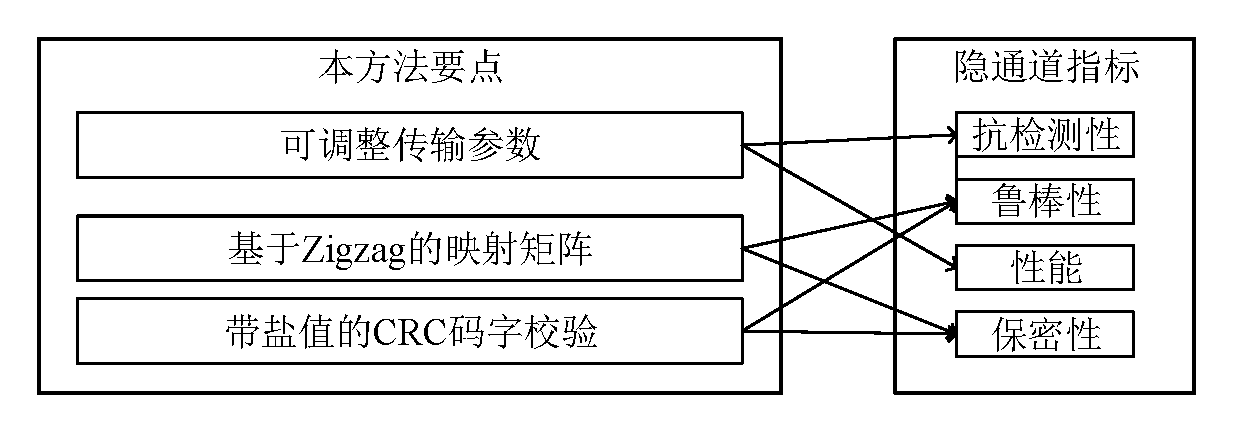
\includegraphics[width=0.8\textwidth]{chapters/chapter4/figures/method-struct.pdf}
        \caption{基于Zigzag映射矩阵的时间隐通道研究要点与指标}
        \label{fig:4:method-struct}
	\end{figure}
}

本章所研究的构建方法,在分片调制的基础上,对每个分片内所传输数据的内容进行调整,提高抗噪声干扰能力。如图\nref{fig:4:method-struct},在鲁棒性方面基于CRC校验,在传输数据码字的过程中穿插校验码字,通过校验信息进行有效数据筛选。在抗检测性方面,参数设置支持不同的$L_{Codeword}$,在Excellent场景与Good场景中对应配置。在保密性方面,引入Zigzag映射矩阵,在码字与符号之间添加一层转换,并且配合初始化参数实现映射矩阵的随机化;同时,在计算CRC校验值时,添加盐值增加结果的随机程度,提高反向破解难度。